Эта часть выполнена Алексеем Биршертом. \\

\subsection{Описание выбранного метода}\label{subsec:описание-метода}
Для предсказания пола и возраста используются две нейронные сети, состоящие из основной и выходной моделей каждая.
В качестве основной модели используется глубокая нейронная сеть ResNet-18, без последнего полносвязного слоя.
В качестве выходной модели используется персептрон из двух полносвязных слоёв с нелинейностью ReLU и дропаутом между ними.
На вход основной модели подаются изображения 227 на 227 пикселей, 3 канала цвета - R, G, B,
выход основной модели подаётся на вход выходной модели.
Выходом нейросети будет выход выходной модели.
Первая нейронная сеть предназначена для классификации пола и имеет в выходной модели 512 и 256 входных и выходных нейронов в первом слое, 256 и 2 во втором соответственно.
Вторая нейронная сеть предназначена для классификации возраста и имеет в выходной модели 512 и 512 входных и выходных нейронов в первом слое, 512 и 101 во втором соответственно.
На вход подаются фотографии лиц людей, выделенные и выровненные с помощью модели детектирования лиц.
Предсказанный пол определяется как номер выходного нейрона соответствующей нейронной сети с максимальным значением -
первый это "женский"\,, второй "мужской".
Предсказанный возраст определяется следующим образом: сначала для вектора значений выходных нейронов
соответсвующей нейронной сети применяется преобразование софтмакс, затем значения умножаются на соответствующий
им возраст.
После вектор суммируется - получаем матожидание возраста при вероятностном распределении, выданном моделью.
\[AGE = \sum\limits_{i = 0}^{100}i \cdot softmax(x)_i, \quad softmax(x)_i = \frac{\exp(x_i)}{\sum\limits_{j =
0}^{100}\exp(x_j)}.\]

\subsection{Описание и подготовка данных}\label{subsec:описание-данных}
В качестве датасета для обучения двух вышеописанных моделей были избраны датасеты IMDB-WIKI-101~\cite{imdb_db} и FGNET~\cite{fgnet}.
Оба датасета имеют в мета-данных метки пола "женщина" или "мужчина"\, и имеют метки возраста в виде целых чисел от 0 до 100 включительно.
Распределение возраста в датасете IMDB-WIKI-101 имеет вид нормальной кривой со средним около 35 лет,
имея малое количество объектов с возрастом меньше 10 лет или больше 90.
Для увеличения количества данных с возрастом до 10 лет был избран датасет FGNET, в котором большая часть объектов это дети до 15 лет.
Для улучшения сходимости нейронных сетей была произведена предобработка всех объектов -
в итоговую выборку не были включены следующие объекты:
объекты с плохо различимыми лицами (показатель уверенности модели распознавания лиц в том, что это лицо, ниже фиксированного значения),
объекты с некорректно заполненными данными по полу/возрасту,
объекты со слишком маленькими фотографиями.
На каждом изображении было выделено и выровнено лицо.
Отступ от границы лица был поставлен на 40\%, чтобы лицо целиком оказывалось на выделенной зоне.
Итого было получено около 200 тысяч объектов, которые были в дальнейшем поделены
с сохранением баланса классов 1 к 19 на валидационную и обучающую выборки соответственно.
\par В качестве датасета для тестирования был избран датасет Adience~\cite{adience}, по которому известно большое количество результатов различных моделей.
Из него были исключены объекты с некорректным описанием пола или возраста.
Итого было получено почти 11 тысяч объектов для тестовой выборки.
В Adience метки возраста в формате 8 групп - 0: [0, 2], 1: [4, 6], 2: [8, 12], 3: [15, 20], 4: [25, 32], 5: [38, 43], 6: [48, 53], 7: [60, 100].
В связи с этим, необходимо было решить как относить к этим группам метки реального возраста от 0 до 100.
Было принято решение относить к той группе, граница которой ближе по модулю, в случае равенства относить к первой в порядке следования.

\subsection{Постановка задач обучения}\label{subsec:постановка-задач-обучения}
Задача классификации пола является задачей бинарной классификации, целевая переменная для одного объекта это число 0 или 1.
Для обучения была выбрана перекрестная энтропия - функция ошибки со следующей формулой:
\[loss(x, y) = -x_y + \log\left(\sum\limits_{j=1}^{K}\exp(x_j)\right),\] где $x$ - вектор значений выходных нейронов нейронной сети,
$y$ - целевая переменная.
Для оценки качества классификации использовались метрика доля правильных ответов, так как выборки сбалансированны по полу.
\par Задача классификации возраста является задачей многоклассовой классификации.
Если смотреть на задачу предсказания возраста по фотографии с точки зрения человека,
человек гораздо точнее способен угадать диапазон возраста, нежели точный возраст.
Поэтому задача классификации возраста была интерпретирована как задача с множественными правильными ответами -
каждому объекту может соответствовать набор правильных классов.
Целевой переменной для одного объекта служил вектор из нулей и единиц, единицы на позициях правильных классов.
Правильные классы определялись как значения возраста, которые отличаются по модулю от правильного не больше,
чем на фиксированное число, которое было гиперпараметром (далее об этом в разделе эксперименты~\ref{subsec:эксперименты}).
Для обучения была выбрана бинарная перекрестная энтропия -
\[loss(x, y) = sum(L), \quad L = \{l_1, \dots l_N\}, \quad l_i = \left(y_i \log(x_i) + (1 - y_i) \log(1 - x_i)\right),\]
где $x$ это вектор значений выходных нейронов нейронной сети после применения сигмоидного преобразования,
$y$ - целевая переменная.
Для оценки качества классификации использовались средний модуль отклонения (далее MAE)
и доля объектов, у которых MAE не превышает фиксированного числа (далее CS-5).

\subsection{Эксперименты}\label{subsec:эксперименты}
В качестве основных было рассмотрено два варианта - нейронная сеть на основе статьи~\cite{ror} и нейронная сеть на основе статьи~\cite{lstm}.
Однако стоит заметить, что анализ и использование модели из второй статьи на порядок сложнее, так как помимо сверточных нейронных сетей там используется блок LSTM,
для работы с которым необходимо иметь соответствующий опыт.
Поэтому было принято решение базировать работу на основе первой статьи, слегка упростив архитектуру.
\par Необходимо было решить вопрос выбора архитектуры базовой модели.
Всего было опробовано три различных архитектуры - MobileNet, ShuffleNet~\cite{shuffle}, ResNet.
Лучше всего себя проявила архитектура ResNet-18.
MobileNet и ShuffleNet незначительно быстрее, не смотря на реализацию, однако достаточно сильно проигрывали в качестве.
В итоге была выбрана архитектура ResNet.
\par Так как ResNet-18 предобучен на датасете ImageNet-1000, он имеет очень хорошую способность выделять признаки из изображения.
Известно, что первые (входные) сверточные слои обученных моделей очень похожи между собой даже для различных задач.
Таким образом, было решено веса первого сверточного слоя ResNet-18 взять из предобученной на ImageNet-1000 модели и заморозить в процессе обучения,
дообучая веса всех остальных слоев.
\par Вторым необходимо было решить вопрос выбора количества моделей - одна нейронная сеть из общей базовой модели и двух паралелльных выходных моделей
или две отдельные нейронные сети из основной и выходной модели.
Однако стоит заметить, что для обеих задач нейронная сеть и должна выделять признаки лица, признаки,
отвечающие за пол, несколько отличаются от признаков, которые соответствуют возрасту.
Также в силу использования функций ошибки,
которые имеют разный масштаб и решают частично разные задачи на моменте основной модели,
и сложности в подборе гиперпараметров для комбинирования этих функций ошибки,
нейронная сеть из одной общей основной модели очень плохо сходилась и достигала намного меньшего качества во всех проведенных экспериментах.
В итоге было принято решение использовать две паралелльные нейронные сети, по одной на решаемую задачу.
\par В процессе подбора гиперпараметров для обучения были выбраны следующие значения: темп обучения был выставлен на $1e-3$ для первых 40 эпох,
далее $1e-4$ для модели предсказания возраста, $1e-4$ для первых 30 эпох и $2e-5$ далее для модели предсказания пола;
коэффициент $L2$ регуляризации был установлен на $1e-3$ для обеих моделей;
размер батча был установлен в силу ограничений на память ГПУ и в качестве дополнительной регуляризации при обучении на 128;
размер входных картинок 227 на 227 пикселей;
дропаут 0.1 перед 4 слоём ResNet, 0.2 перед первым полносвязным слоём и 0.4 между слоями.
В качестве размера окна для правильного возраста после сравнений было выбрано число в 5 лет.
Модели, обученные с такими гиперпараметрами показали наилучшие результаты.
\par В процессе выбора аугментации были выбраны следующие трансформации -
в процессе обучения при проходе по датасету каждое изображение преобразовывалось к квадрату 256 на 256 пикселей,
затем из него выбирался случайный квадрат со стороной 227 пикселей,
который с вероятностью $1/2$ мог быть отражен вдоль вертикальной оси, проходящей через его центр.
Во время тестирования каждое изображение преобразовывалось к квадрату 256 на 256 пикселей,
затем из него по центру вырезался квадрат со стороной 227 пикселей.

\subsection{Результаты}\label{subsec:результаты}
Как итог модели показали следующие показатели метрик на обучающей и валидационной выборках: для возраста MAE 5 и 5.6 соответственно,
CS-5 0.71 и 0.69 соответственно, для пола Accuracy 0.94 и 0.93 соответственно.
\par Модель показала следующие результаты на датасете Adience: для возраста Exact-accuracy $49.1\% \pm 4.1 \%$ и One-off-accuracy $84.4\% \pm 3.6 \%$,
для пола значение метрики Accuracy $83.7\% \pm 2.7\%$.
Значения метрик получаются подсчетом соответствующих метрик для каждой из 8 возрастных групп
и вычисления среднего арифметического от посчитанных показателей.
\par Всего было написано более 2300 строк кода на языке программирования Python3,
все модели были написаны и обучены с использованием фреймворка машинного обучения PyTorch.
\newpage

\subsection{Примеры работы модели}\label{subsec:примеры-работы-модели2}
\begin{figure}[h!]
    \centering
    \begin{subfigure}[b]{1.02\linewidth}
        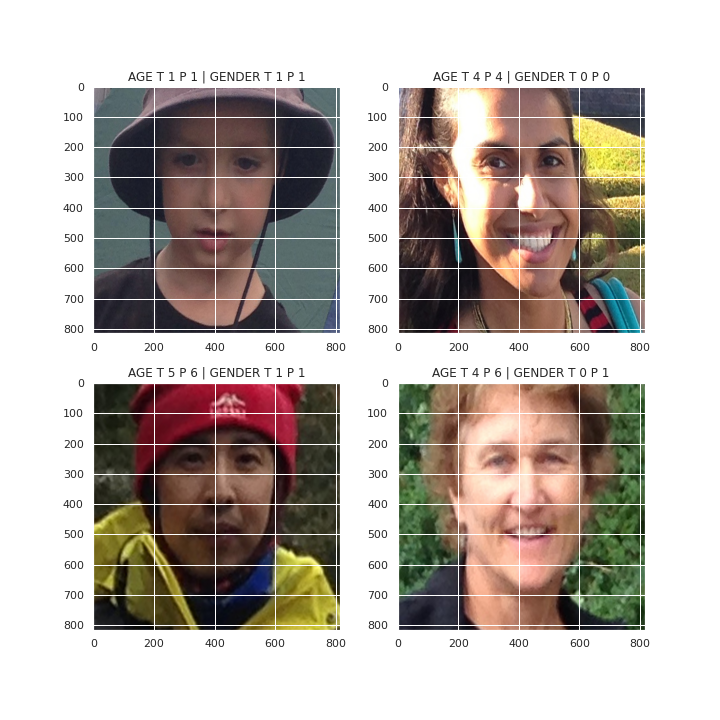
\includegraphics[width=\linewidth]{images/image.png}
        \caption{Пример ответов модели на 4 разных лицах}
    \end{subfigure}
\end{figure}
Здесь мы видим примеры ответов модели на случайных изображениях из датасета Adience.
Для каждого изображения написана информация про правильный ответ и ответ модели по следующему формату -
сначала идёт название целевой переменной, потом правильный ответ после метки \textbf{T}, потом ответ модели после метки \textbf{P}.
Напомним, что метки пола имеют соответствие 0 - "женщина"\,, 1 - "мужчина"\,.
Метки возраста - 0: [0, 2], 1: [4, 6], 2: [8, 12], 3: [15, 20], 4: [25, 32], 5: [38, 43], 6: [48, 53], 7: [60, 100].